\section{Expressiveness} 

\label{app:expressivity}

We argue the expressiveness of our approach by comparing with example specifications  proposed in \cite{OOPSLA22,dd,irisWasm23}.

\subsection{The DOM}  %\sophiaPonder[renamed Wrapper to Proxy]{  
\label{ss:DOM}
This is the motivating example in \cite{dd}. It
deals with a tree of DOM nodes: Access to a DOM node
gives access to all its \prg{parent}s, % simoplified it and \prg{children} nodes, 
with the ability to modify the node's contents   -- where  \prg{parent} %\prg{children} 
and \prg{cnt} are fields in class \prg{Node}. Since the top nodes of the tree
usually contain privileged information, while the lower nodes contain
less crucial third-party information, we must be able to limit 
 access given to third parties to only the lower part of the DOM tree. 
 
To do this,   \citet{dd}  propose   
  a \prg{Proxy} class, which has a field \prg{node} pointing to a \prg{Node}, and a field height (\prg{hght}), which restricts the range of \prg{Node}s which may be modified through the use of the particular \prg{Proxy}. Namely,   a \prg{Proxy}  may modify 
the \prg{cnt} of all the ancestors of its  \prg{node}, up to the   \prg{hght}-th ancestor of that \prg{node}. 

A possible implementation of such \prg{Node} and \prg{Proxy} classes is shown in Fig.  \ref{fig:DoMCode}, 
while the creation of a tree, three proxies, and  passing the proxies to the external world is shown in Fig \ref{fig:DoMCodeClient}.

\begin{figure}[tbh]
\begin{lstlisting}[language = Chainmail, mathescape=true, frame=lines]
module DOM 
   class Node
      field cnt: int
      field parent: Node 
      
   class Proxy
      field hght: nat
      field node: Node
	
      public method set(newCnt:int, up:nat): void
            if this.hght >= up
                  setPrivate(newCnt, up)
            else
                  return
	       
      private method setPrivate(newCnt:int, up:nat): void
            if up==0 then
                  this.node.cnt := nwCnt
            else
                  setPrivate(newCnt, up-1)
\end{lstlisting}
\caption{The DOM module  -- classes \prg{Node} and \prg{Proxy}}
\label{fig:DoMCodeClient}
\end{figure}


We now discuss possible specifications. For this, we will use  the predicate $may\_modify \subseteq \prg{Proxy} \times \prg{Node}$, which says that 
\prg{prx} has \emph{modification-capabilities} on \prg{nd}, where \prg{prx} is
a  \prg{Proxy} and \prg{nd} is a \prg{Node}, if \prg{nd} is the \prg{prx}$k^{th}$  parent
of   \prg{pr.node} where $k \leq \prg{nd}.\prg{hght}$.
The formal definition is as follows:
\\
$\strut \SPSP   may\_modi\!f\!y(\prg{prx}, \prg{nd}) \triangleq \exists k:\mathbb{N}. [ \  \prg{prx}.\prg{node}.\prg{parent}^k=\prg{nd}\ \wedge k\leq   \prg{prx}.\prg{hght}]$
\\
Thus, a \prg{Proxy} object \prg{prx}, which satisfies $may\_modi\!f\!y(\prg{prx},\prg{nd})$ is a capability which may modify the node $\prg{nd}$. 


\begin{figure}[tbh]
\begin{lstlisting}[language = Chainmail, mathescape=true, frame=lines]
module DOM 
   ... as before ...
   class Example
      public method demo(untrst:external) : void 
          //  create a tree of  $\prg{Node}s$
         nd1 := new Node; nd1.cnts := 1
         nd2 := new Mode; nd2.parent:= nd1; nd2,ctns:=2;
         nd3 := new Mode; nd3.parent:= nd1; nd3,ctns:=3;
         nd4 := new Mode; nd4.parent:= nd2; nd4,ctns:=4;
         nd5 := new Mode; nd5.parent:= nd2; nd5,ctns:=5;
         
         //  create three $\prg{Proxy}s$
         prx10 := newProxy; prx10.height:=2; prx10.node:=nd4;
         prx11 := newProxy; prx10.height:=1; prx10.node:=nd4; 
         prx12 := newProxy; prx10.height:=0; prx10.node:=nd4;
          
         untrst.meth_A(); //  1st external call  
         // no modification in the tree
         
         untrst.meth_B(nd2); //  2nd external call  
         // no modification in the tree     
         
         untrst.meth_C(prx12); //  3rd external call  
         // nd4.cnts may have changed; 
         // all else has stayed the same
         
         nd4.ctns:=4  // re-establish old value of nd4.ctns
         untrst.meth_A( ); //  4th external call  
         // nd4.cnts may have changed again; 
         // all else has stayed the same
         
         untrst.meth_C(prx10);
        // nd4.cnts, nd2.cnts, nd1.ctns may have changed; 
        // all else has stayed the same          
\end{lstlisting}
\caption{The DOM module continued -- class \prg{Example} }
\label{fig:DoMCodeClient}
\end{figure}

In Fig. \ref{f:DOM:Diagrs} in the left-most pane we see a tree consisting of the five nodes, \prg{nd1}, \prg{nd2},  \prg{nd3} and \prg{nd4}, 
and the three proxies, \prg{prx10}, \prg{prx11},  and \prg{prx12}, created in lines 6-15 in the code in Fig. \ref{fig:DoMCodeClient}.

\begin{figure}[th] 
\begin{tabular}{|c|c|c|}
\hline
\resizebox{3,5cm}{!}{
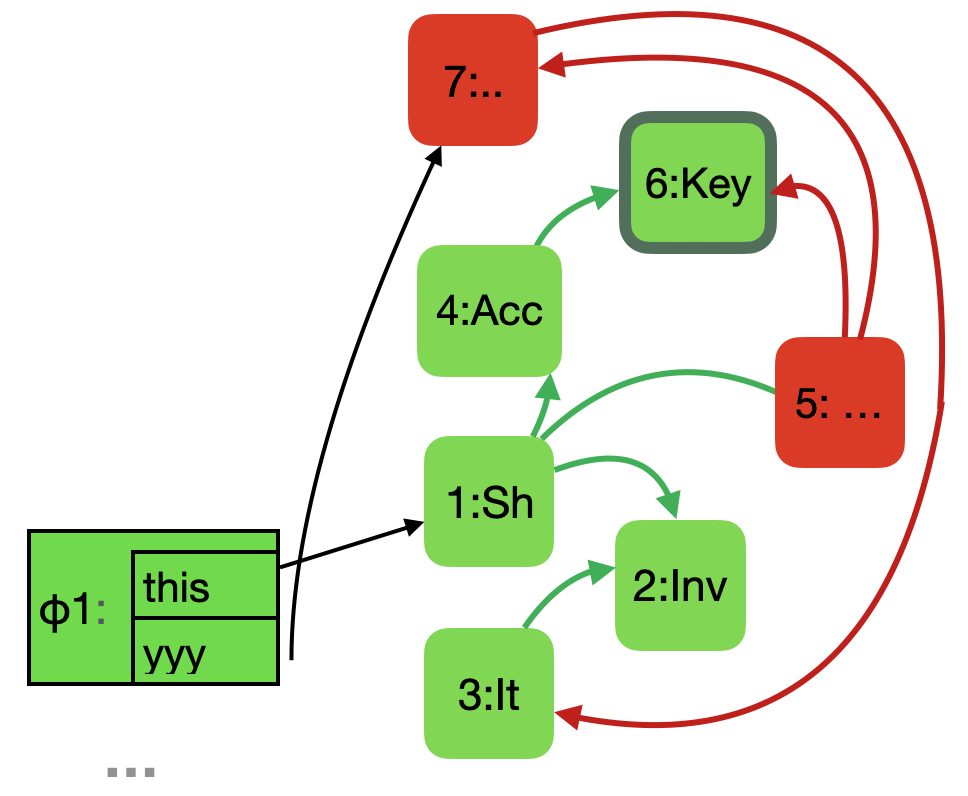
\includegraphics[width=\linewidth]{diagrams/ShopB.png}
} 
&
\resizebox{3,5cm}{!}{
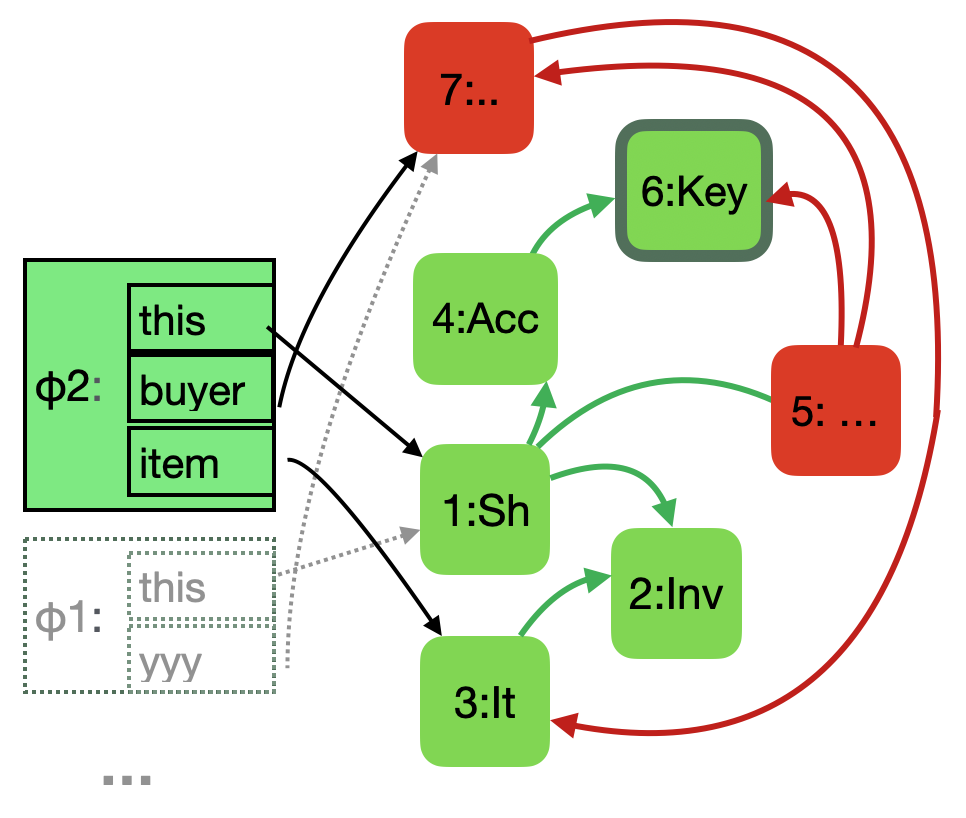
\includegraphics[width=\linewidth]{diagrams/ShopC.png}
}
&
\resizebox{3.5cm}{!}{
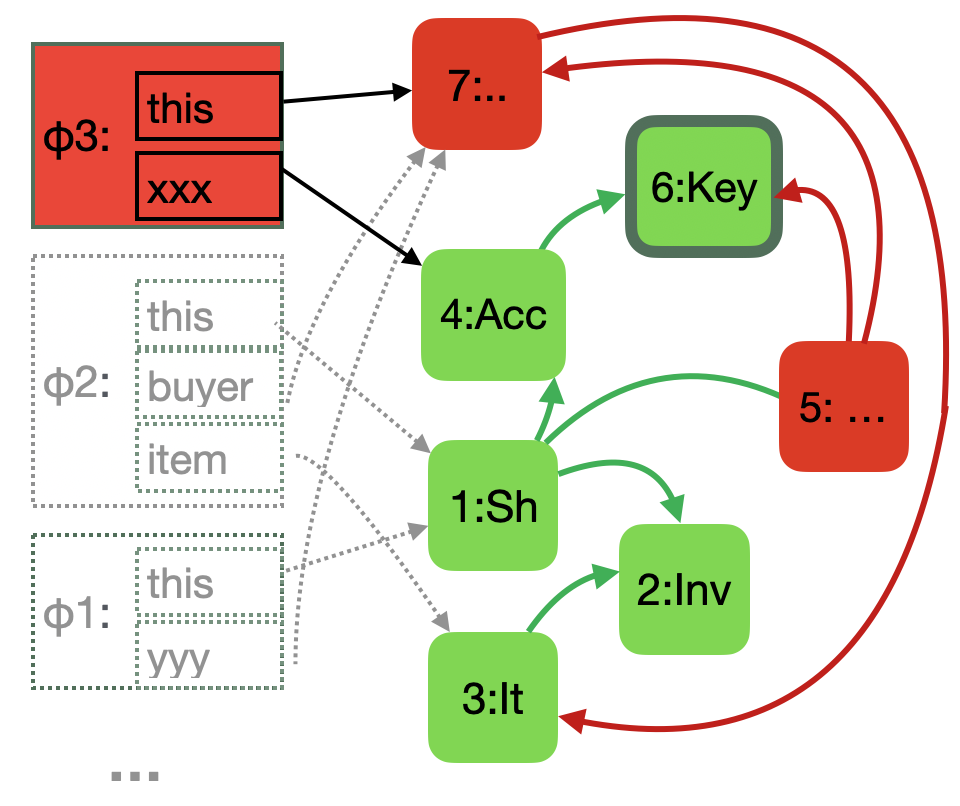
\includegraphics[width=\linewidth]{diagrams/ShopD.png}
}
\\ 
\hline % \hline
\end{tabular}
\caption{DOM trees and Proxies}
 \label{f:DOM:Diagrs}
 \end{figure}
 
 
\vspace{.1cm}

\noindent
We now discuss propose three specifications:
\ \ 
Below, $S_{dom\_1}$ mandates  that nodes, $\prg{nd}$ are not leaked. 
\\
$\strut \SPSP  S_{dom\_1}\ \  \triangleq \ \ \TwoStatesN{ \prg{nd}:\prg{Node}}{\  \inside{\prg{nd}}\  ] \ }$ 
\\
\noindent
{Also, $S_{dom\_2}$ mandates  that proxies which $may\_modi\!f\!y(\prg{prx},\prg{nd})$ are not leaked.}
\\
$\strut \SPSP  S_{dom\_2}\ \  \triangleq \ \ \TwoStatesN{ \prg{nd}:\prg{Node}}{\  \forall \prg{prx}:\prg{Proxy}.[ \ may\_modi\!f\!y(\prg{prx}, \prg{nd}) \rightarrow \inside{\prg{prx}}\  ] \ }$ 
\\
{Finally, $S_{dom\_3}$ mandates   that proxies which $may\_modi\!f\!y(\prg{prx},\prg{nd})$ are not leaked, and that when a node $nd$ is protected, and  all proxies that can  $may\_modi\!f\!y(\prg{prx},\prg{nd})$ are protected, then  the $cnt$ of $nd$ cannot be modified by external code.}
\\
$\strut \SPSP  S_{dom\_3}\ \  \triangleq \ \  \forall{ \prg{nd}:\prg{Node}.\forall \prg{val}:\prg{Object} }$.\\
$\strut \SPSP\strut  \SPSP\strut \SPSP	\{  \  \inside{\prg{nd}} \wedge \forall \prg{prx}:\prg{Proxy}.[ \ may\_modi\!f\!y(\prg{prx}, nd) \rightarrow \inside{\prg{prx}}\  ]  \wedge \prg{nd.cnt} = \prg{val} \ \}  $ 


Note that $S_{dom\_3}$ is strictly stronger than $S_{dom\_2}$. 
The module shown in Fig. \ref{fig:DoMCode}, and \ref{fig:DoMCodeClient} does satisfies all three specifications from above. 
\footnote{The careful reader might worry that the method \prg{demo} in class \prg{Example} in Fig. \ref{fig:DoMCodeClient} 

}
Also,  $S_{dom\_3}$ is needed 
for the proof of the preservation of the  values \prg{cnt}, as shown in the client in Fig. \ref{fig:DoMCodeClient}, while  



\vspace{.1cm}

\citet{OOPSLA22} specify this as:
 
 \begin{lstlisting}[language = Chainmail, mathescape=true, frame=lines]
DOMSpec $\triangleq$ from nd : Node $\wedge$ nd.property = p  to nd.property != p
  onlyIf $\exists$ o.[ $\external {\prg{o}}$ $\wedge$ 
     $( \exists$ nd':Node.[ $\access{\prg{o}}{\prg{nd'}}$ ]  $\vee$ 
     $\,\;\exists$ pr:Proxy,k:$\mathbb{N}$.[$\, \access{\prg{o}}{\prg{pr}}$ $\wedge$ nd.parent$^{\prg{k}}$=pr.node.parent$^{\prg{pr.height}}$ ] $\,$ ) $\,$ ]
\end{lstlisting}

\prg{DomSpec} states that the \prg{property} of a node can only change if
some external object presently has 
access to a node of the DOM tree, or to some \prg{Proxy} with modification-capabilties
to the node that was modified.
The assertion $\exists {o}.[\ \external {\prg{o}} \wedge \access{\prg{o}}{\prg{pr}}\ ]$ is the contrapositive of our  $\inside{pr}$, but is is weaker than that, because it does not specify the frame from which $o$ is accessible.
Therefore, $\prg{DOMSpec}$ is a stronger requirement than $S_{dom\_1}$.

In Fig. \ref{fig:DoMCode} for a module that satisfies such a specification. 






% \pagebreak 
\subsection{DAO}
The Decentralized Autonomous Organization (DAO)~\cite{Dao}  is a well-known Ethereum contract allowing 
participants to invest funds. The DAO famously was exploited with a re-entrancy bug in 2016, 
and lost \$50M. Here we provide specifications that would have secured the DAO against such a 
bug. 
\\ 
$\strut \SPSP  S_{dao\_1}\ \  \triangleq \ \ \TwoStatesN{ d:\prg{DAO}}{\ \forall p:\prg{Participant}. [\ d.ether \geq d.balance(p) \ ]   \ }$ 
\\
$\strut \SPSP  S_{dao\_2}\ \  \triangleq \ \ \TwoStatesN{ d:\prg{DAO}}{\ \ d.ether \geq \sum_{p \in d.particiants} d.balance(p)\  \ }$ 


The specifications above say the following:
\\
\begin{tabular}{ll}
\begin{minipage}{.10\textwidth}
$\strut \SPSP  S_{edao\_1}$
\end{minipage}
&
\begin{minipage}{.85\textwidth}
guarantees that the DAO holds more ether than the balance  of any of its  participant's.
\end{minipage}
\\
\\
\begin{minipage}{.10\textwidth}
$\strut \SPSP  S_{dao\_2}$ 
\end{minipage}
&
\begin{minipage}{.85\textwidth}
guarantees that that the DAO holds more ether than the sum  of the balances held by DAO's participants.
\end{minipage}
\end{tabular}

$S_{dao\_2}$  is stronger than $S_{dao\_1}$. They would both have precluded the DAO bug. Note that these specifications  do not mention capabilities. 
They are, essentially, simple class invariants and could have been expressed with the techniques proposed already by \cite{MeyerDBC92}.
The only difference is that $S_{dao\_1}$ and $S_{dao\_2}$ are two-state invariants, which means that we require that they are \emph{preserved},
\ie if they hold in one (observable) state they have to hold in all successor states,
while class invariants are one-state, which means they are required to hold in all (observable) states.
\footnote{This should have been explained somewhere earlier.}

\vspace{0.5cm}
We now compare with the specification given in \cite{OOPSLA22}.
\prg{DAOSpec1} in similar to  $S_{dao\_1}$: iy
says that no participant's balance may ever exceed the ether remaining 
in DAO. It is, essentially, a one-state invariant.


\begin{lstlisting}[language = Chainmail, mathescape=true, frame=lines]
DAOSpec1 $\triangleq$ from d : DAO $\wedge$ p : Object
            to d.balance(p) > d.ether
            onlyIf false
\end{lstlisting}
\prg{DAOSpec1}, similarly to $S_{dao\_1}$,   in that it enforces a class invariant of \prg{DAO}, something that could be enforced
by traditional specifications using class invariants.


 \cite{OOPSLA22}  gives one more   specification: 
 
 \begin{lstlisting}[language = Chainmail, mathescape=true, frame=lines]
DAOSpec2 $\triangleq$ from d : DAO $\wedge$ p : Object
            next d.balance(p) = m
            onlyIf $\calls{\prg{p}}{\prg{d}}{\prg{repay}}{\prg{\_}}$ $\wedge$ m = 0 $\vee$ $\calls{\prg{p}}{\prg{d}}{\prg{join}}{\prg{m}}$ $\vee$ d.balance(p) = m
\end{lstlisting}

 \prg{DAOSpec2} states that if after some single step of execution, a participant's balance is \prg{m}, then 
either 
\begin{description}
\item[(a)] this occurred as a result of joining the DAO with an initial investment of \prg{m}, 
\item[(b)] the balance is \prg{0} and they've just withdrawn their funds, or 
\item[(c) ]the balance was \prg{m} to begin with
\end{description}

%\subsection{Safe}
%\cite{FASE} used as a running example   a Safe, where a treasure 
%was secured within a \texttt{Safe} object, and access to the treasure was only granted by 
%providing the correct password. 
%\red{Sophia proposes that we drop the Safe}
%\ Using \Nec, we express \texttt{SafeSpec}, that requires that the treasure cannot be 
%removed from the safe without knowledge of the secret.
%\begin{lstlisting}[language = Chainmail, mathescape=true, frame=lines]
%SafeSpec $\triangleq$ from s : Safe $\wedge$ s.treasure != null
%            to s.treasure == null
%            onlyIf $\neg$ inside(s.secret)
%\end{lstlisting}
%
%The module  \prg{SafeModule} described  below satisfies  \prg{SafeSpec}.
%
%\begin{lstlisting}[frame=lines]
%module SafeModule
%     class Secret{}
%     class Treasure{}
%     class Safe{
%         field treasure : Treasure
%         field secret : Secret
%         method take(scr : Secret){
%              if (this.secret==scr) then {
%                   t=treasure
%                   this.treasure = null
%                   return t } 
%          }
% }
%\end{lstlisting}

\subsection{ERC20}

The ERC20 \cite{ERC20} is a widely used token standard describing the basic functionality of any Ethereum-based token 
contract. 
This functionality includes issuing tokens, keeping track of tokens belonging to participants, and the 
transfer of tokens between participants. Tokens may only be transferred if there are sufficient tokens in the 
participant's account, and if either they (using the \prg{transfer} method) or someone authorised by the participant (using the \prg{transferFrom} method) initiated the transfer. 

For an $e:\prg{ERC20}$, the term $e.balance(p)$  indicates the number of tokens in   participant $p$'s  account at $e$.
The 
assertion $e.allowed(p,p')$ expresses that participant $p$ has been authorised to spend moneys from $p'$'s account at $e$.
 
The security model in Solidity is not based on having access to a capability, but on who the caller of a method is. 
Namely, Solidity supports the  construct \prg{sender} which indicates the identity of the caller.
Therefore, for Solidity, we adapt our approach in two significant ways:
we change the meaning of $\inside{\re}$ to express that $\re$ did not make a method call.
Moreover, we introduce a new, slightly modified form of two state invariants of the form $\TwoStates{\overline {x:C}}{A}{A'}$ which expresses that any execution which satisfies $A$, will preserve $A'$.
% \footnote{\red{I think that something deeper is going on here, I think that SOLIDITY id more in the style of ACLs, than OCAPs.}}

% \footnote{\red{AUTHORS: the way we had written the spec of ECR20 at OOPSLA, the tokens are taken out of the ERC20 and just disappear rather than being transferred to a another account. Was that correct?{ It would be easy to change}}}

We specify the guarantees of   ERC20  as follows:
\\
ç
\\
$\strut \SPSP  S_{erc\_2}\ \  \triangleq \ \ \TwoStatesLB{ e:\prg{ERC20},p,p':\prg{Participant},n:\mathbb{N}} 
 {\ \forall p'.[\,(e.allowed(p',p) \rightarrow   \inside{p'}\, ] \ } { \ e.balance(b)=n \ } $ 
\\
$\strut \SPSP  S_{erc\_3}\ \  \triangleq \ \ \TwoStatesLB{ e:\prg{ERC20},p,p':\prg{Participant}}  {\ \forall p'.[\,(e.allowed(p',p) \rightarrow   \inside{p'}\, ] \ } { \ \neg (e.allowed(p'',p) \ } $ 

The specifications above say the following:
\\
\begin{tabular}{ll}
\begin{minipage}{.10\textwidth}
$\strut \SPSP  S_{erc\_1}$
\end{minipage}
&
\begin{minipage}{.85\textwidth}
guarantees that the the owner of an account is always authorized on that account -- this specification is expressed using the original version of two-state invariants.
\end{minipage}
\\
\\
\begin{minipage}{.10\textwidth}
$\strut \SPSP  S_{erc\_2}$ 
\end{minipage}
&
\begin{minipage}{.85\textwidth}
guarantees that any execution which does not contain calls from a participant $p'$ authorized on $p$'s account will not affect the balance of $e$'s account. Namely, if the execution starts in a state in which $ e.balance(b)=n$, it will lead to a state where $ e.balance(b)=n$ also holds.
\end{minipage}
\\
\\
\begin{minipage}{.10\textwidth}
$\strut \SPSP  S_{erc\_3}$ 
\end{minipage}
&
\begin{minipage}{.85\textwidth}
guarantees that any execution which does not contain calls from a participant $p'$ authorized on $p$'s account will not affect who else is authorized on that account. That is, if the execution starts in a state in which $ \neg (e.allowed(p'',p)$, it will lead to a state where $ \neg (e.allowed(p'',p)$ also holds.
\end{minipage}
\end{tabular}

%$\strut \SPSP  S_{erc\_1}$ guarantees that the the owner of an account is always authorized on that account -- this specification is expressed using the original version of two-state invariants.
%\\
%$\strut \SPSP  S_{erc\_2}$ guarantees that any execution which does not contain calls from a participant $p'$ authorized on $p$'s account will not affect the balance of $e$'s account. Namely, if the execution starts in a state in which $ e.balance(b)=n$, it will lead to a state where $ e.balance(b)=n$ also holds.
%\\
%$\strut \SPSP  S_{erc\_3}$ guarantees that any execution which does not contain calls from a participant $p'$ authorized on $p$'s account will not affect the balance of $e$'s account. That is, f the execution starts in a state in which $ \neg (e.allowed(p'',p)$, it will lead to a state where $ \neg (e.allowed(p'',p)$ also holds.

\vspace{1cm}

We compare with the specifications given in \cite{OOPSLA22}:
 Firstly, \prg{ERC20Spec1} 
says that if the balance of a participant's account is ever reduced by some amount $m$, then
that must have occurred as a result of a call to the \prg{transfer} method with amount $m$ by the participant,
or the \prg{transferFrom} method with the amount $m$ by some other participant.
\begin{lstlisting}[language = Chainmail, mathescape=true, frame=lines]
ERC20Spec1 $\triangleq$ from e : ERC20 $\wedge$ e.balance(p) = m + m' $\wedge$ m > 0
              next e.balance(p) = m'
              onlyIf $\exists$ p' p''.[$\calls{\prg{p'}}{\prg{e}}{\prg{transfer}}{\prg{p, m}}$ $\vee$ 
                     e.allowed(p, p'') $\geq$ m $\wedge$ $\calls{\prg{p''}}{\prg{e}}{\prg{transferFrom}}{\prg{p', m}}$]
\end{lstlisting}
Secondly, \prg{ERC20Spec2} specifies under what circumstances some participant \prg{p'} is authorized to 
spend \prg{m} tokens on behalf of \prg{p}: either \prg{p} approved \prg{p'}, \prg{p'} was previously authorized,
or \prg{p'} was authorized for some amount \prg{m + m'}, and spent \prg{m'}.
\begin{lstlisting}[language = Chainmail, mathescape=true, frame=lines]
ERC20Spec2 $\triangleq$ from e : ERC20 $\wedge$ p : Object $\wedge$ p' : Object $\wedge$ m : Nat
              next e.allowed(p, p') = m
              onlyIf $\calls{\prg{p}}{\prg{e}}{\prg{approve}}{\prg{p', m}}$ $\vee$ 
                     (e.allowed(p, p') = m $\wedge$ 
                      $\neg$ ($\calls{\prg{p'}}{\prg{e}}{\prg{transferFrom}}{\prg{p, \_}}$ $\vee$ 
                              $\calls{\prg{p}}{\prg{e}}{\prg{allowed}}{\prg{p, \_}}$)) $\vee$
                     $\exists$ p''. [e.allowed(p, p') = m + m' $\wedge$ $\calls{\prg{p'}}{\prg{e}}{\prg{transferFrom}}{\prg{p'', m'}}$]
\end{lstlisting}
%\end{example}

\prg{ERC20Spec1} is related to $S_{erc\_2}$. Note that \prg{ERC20Spec1} is more API-specific, as it expresses the precise methods which caused the modification of the balance.

\subsection{Wasm, Iris, and the stack}

%
In \cite{irisWasm23}, they consider inter-language safety for Wasm. They develop Iris-Wasm, a mechanized higher-order separation logic mechanized in Coq and the Iris framework. Using Iris-Wasm, with the aim to
specify and verify individual modules separately, and then compose them modularly in a simple host language
featuring the core operations of the WebAssembly JavaScript Interface. They develop a 
logical relation that enforces robust safety: unknown, adversarial code can only affect other modules through
the functions that they explicitly export. 
They do not offer however a logic to deal with the effects of external calls.

As a running example, they use a \prg{stack} module, which is an array of values, and exports functions to inspect the stack contents or modify its contents. 
Such a setting can be expressed in our language through a \prg{stack} and a \prg{modifier} capability.
Assuming a predicate $Contents(\prg{stack},\prg{i},\prg{v})$, which expresses that the contents of \prg{stack} at index \prg{i} is \prg{v}, we can specify the stack through
 
 $$\strut \SPSP  S_{stack}\ \  \triangleq \ \ \TwoStatesN{ s:\prg{Stack},i:\mathbb{N},\prg{v}:\prg{Value}} 
 {\ \inside{\prg{s.modifier}} \ \wedge \ Contents(\prg{s},i,\prg{v})\  }$$  
 
 
 
 In that work, they provide a tailor-made proof that indeed, when the stack makes an external call, passing only the inspect-capability, the contents will not change. 
 However, because the language is essentially functional, they do not consider the possibility that the external call might already have stored the modifier capability.
 Moreover, the proof does not make use of a Hoare logic.  
 
 \subsection{Sealer-Unsealer pattern} 
 The sealer-unsealer pattern, proposed by \citet{JamesMorris}, is a security  pattern  to enforce data
abstraction while interoperating with untrusted  code. He proposes a function
\prg{makeseal} which generating pairs of functions (\prg{seal}, \prg{unseal} ), such that \prg{seal} takes a value $v$ and returns a low-integrity value $v'$.
The function \prg{unseal} when given $v'$ will return $v$. But there is no other way to obtain $v$ out of $v'$ except throughthe use of the \prg{usealer}.
Thus, $v'$ can securely be shared with untrusted code.
This pattern has been studied by \citet{ddd}.

We formulate this pattern here. 
As we are working with an object oriented rather than a functional language, we assume the existence of a class 
\prg{DynamicSealer} with two methods, \prg{seal}, and \prg{unseal}. 
And we define a predicate $Sealed(v,v',us)$ to express that $v$ has been sealed into $v'$ and can be unsealed using $us$.

Then, the scoped invariants 

 $$\strut \SPSP  S_{sealer\_1}\ \  \triangleq \ \ \TwoStatesN{ \prg{v},\prg{v}',\prg{us}: \prg{Object} }
 {\   \inside{\prg{us}} \ \wedge\ Sealed(\prg{v},\prg{v}',\prg{us}) }$$  
 
 $$\strut \SPSP  S_{sealer\_2}\ \  \triangleq \ \ \TwoStatesN{ \prg{v},\prg{v}',\prg{us}: \prg{Object} }
 {\ \inside{\prg{v}} \ \wedge \ \inside{\prg{us}} \ \wedge\ Sealed(\prg{v},\prg{v}',\prg{us}) }$$  

\noindent
 expresses that the unsealer is not leaked to external code ($S_{sealer\_1}$), and that if the external world has no access to the high-integrity value $\prg{v}$ nor to the its unsealer  \prg{us}, then it will not get access to the value  ($S_{sealer\_2}$). 

%
%Moreover, we would add method specifications to the \prg{seal}, and \prg{unseal} methods as follows, where $res.1$ and $res.2$ stand for taking the 1st or 2nd element out of a tuple.
%
%  {\sprepost
%		{\strut \ \ \ \ \ \ \ \ \ S_{sealer\_seal}} 
%		{  v, o:\prg{Object \wedge  \inside{o} }
%		{\prg{public DynamicSealer}} {\prg{seal}} {\prg{v}:\prg{Object}}
%		{   \inside{o}\wedge\ Sealed(v, res.1, res.2) \wedge   \inside{res.2}}
%		{   \inside{o}  \wedge   \inside{res.2} }
%}}
%
% 
%  {\sprepost
%		{\strut \ \ \ \ \ \ \ \ \ S_{sealer\_unseal\_1}} 
%		{ \prg{v'}, o:\prg{Object} \wedge  \inside{o} \wedge\ Sealed(v, \prg{v'}, \prg{us}) \wedge \prg{us}=\preg{us}' }
%		{\prg{public DynamicSealer}} {\prg{unseal}} {\prg{v'}:\prg{Object}, \prg{us'}:\prg{Object}}
%		{ \   Sealed(v, \prg{v'}, \prg{us}) \wedge res=\prg{v} }
%		{   \inside{o} }
%}
%
%
%{\sprepost
%  {\strut \ \ \ \ \ \ \ \ \ S_{sealer\_unseal\_2}}
%                  { \prg{v'}, o:\prg{Object} \wedge  \inside{o} \wedge\ Sealed(v, \prg{v'}, \prg{us}) \wedge \prg{us}\neq\preg{us}' }
%		{\prg{public DynamicSealer}} {\prg{unseal}} {\prg{v'}:\prg{Object}, \prg{us'}:\prg{Object}}
%		{ \   Sealed(v, \prg{v'}, \prg{us}) \wedge res=\preg{v}' }
%		{   \inside{o} }
%}





%\subsection{Crowdsale}
\jm[]{\Nec is able to encode the motivating example of \citeasnoun{VerX}: 
an escrow smart contract that ensures that the contract may not be coerced to 
pay out or refund more money than has been raised.
The motivating \prg{Crowdsale} example consists of a \prg{Crowdsale} contract 
for crowd sourcing funding. A \prg{Crowdsale} object consists of an \prg{Escrow} object,
an amount raised, a funding goal, and a closing time in which the goal must be met for 
the fund to be successful. An \prg{Escrow} consists of a ledger of investors and how much
they have invested. There are several properties that \citeasnoun{VerX} sought to encode,
and we have provided the encoding of those specifications in Fig. \ref{f:verx:encoding}.
\prg{R0} states that if an investor claims a refund from an escrow, then the balance of 
the escrow decreases by the amount the investor had deposited in the escrow. 
\prg{R1} states that if at anytime the escrow has not yet succeeded, then the deposits must
be less than the balance of the escrow. 
\prg{R2\_1} and \prg{R2\_2} combine to express a single property: no one may ever withdraw and 
then subsequently claim a refund or visa versa.
\prg{R3} states that if the funding goal is ever met, then no one may subsequently claim a refund.}

\begin{figure}[htb]
\begin{lstlisting}[language=chainmail]
class Crowdsale {
Escrow escrow;
  closeTime, raised, goal : int;
  method init() {
    if escrow == null
      escrow := new Escrow(new Object);
    	  closeTime := now + 30 days;
    	  raised := 0;
    	  goal := 10000 * 10**18;
  }
  method invest(investor : Object, value : int) {
    if raised < goal
      escrow.deposit(investor, value);
      raised += value;
  }
  method close() {
    if now > closeTime || raised >= goal
      if raised >= goal
        escrow.close();
      else
        escrow.refund();
  }
}
\end{lstlisting}
\caption{Crowdsale Contract}
\label{f:verx:crowdsale}
\end{figure}

\begin{figure}[htb]
\begin{lstlisting}[language=chainmail]
confined class Escrow {
  owner, beneficiary : Object;
  mapping(Object => uint256) deposits;
  OPEN, SUCCESS, REFUND : Object;
  state : Object;
  method init(o : Object, b : Object) {
    if owner == null || beneficiary == null
      owner := o;
      beneficiary := b;
      OPEN := new Object; SUCCESS := new Object; REFUND := new Object;
      state := OPEN;
      
  method close() {state = SUCCESS;}
  method refund() {state = REFUND;}
  method deposit(value : int, p : Object) {
    deposits[p] := deposits[p] + value;
  }
  method withdraw() {
    if state == SUCCESS
      return this.balance;
  }
  method claimRefund(p : Object) {
    if state == REFUND
      int amount := deposits[p];
      deposits[p] := 0;
      return amount;
  }
}
\end{lstlisting}
\caption{Escrow Contract}
\label{f:verx:escrow}
\end{figure}

\begin{figure}[htb]
\begin{lstlisting}[mathescape=true, language=chainmail]
(R0) $\triangleq$ e : Escrow $\wedge$ $\calls{\_}{\prg{e}}{\prg{claimRefund}}{\prg{p}}$
          next e.balance = nextBal onlyIf nextBal = e.balance - e.deposits(p)
(R1) $\triangleq$ e : Escrow $\wedge$ e.state $\neq$ e.SUCCESS $\longrightarrow$ sum(deposits) $\leq$ e.balance
(R2_1) $\triangleq$ e : Escrow $\wedge$ $\calls{\_}{\prg{e}}{\prg{withdraw}}{\prg{\_}}$
           to $\calls{\_}{\prg{e}}{\prg{claimRefund}}{\prg{\_}}$ onlyIf false
(R2_2) $\triangleq$ e : Escrow $\wedge$ $\calls{\_}{\prg{e}}{\prg{claimRefund}}{\prg{\_}}$
           to $\calls{\_}{\prg{e}}{\prg{withdraw}}{\prg{\_}}$ onlyIf false
(R3) $\triangleq$ c : Crowdsale $\wedge$ sum(deposits) $\geq$ c.escrow.goal
         to $\calls{\_}{\prg{c.escrow}}{\prg{claimRefund}}{\prg{\_}}$ onlyIf false
\end{lstlisting}
\caption{Encoding VerX Crowdsale Example in Necessity}
\label{f:verx:encoding}
\end{figure}

